\documentclass{cours}

\title{Orthogonalité dans l'Espace}

\begin{document}
    \maketitle{12}

    \begin{Gpartie}{Différentes Expressions du Produit Scalaire} 
        \vspace{-2ex}
        \begin{Spartie}{Définitions} 
            $\vec{u}$ et $\vec{v}$ étant deux vecteurs de l'espace, soit un point $A$ de l'espace, et les points $B$ et $C$ tels que $\overrightarrow{AB}=\vec{u}$ et $\overrightarrow{AC}=\vec{v}$.

            Alors, $\vec{u}\cdot\vec{v}=\overrightarrow{AB}\cdot\overrightarrow{AC}$\quad(Produit Scalaire de deux vecteurs dans le plan (ABC))

            Ainsi, toutes les définitions et propriétés du produit scalaire dans le plan sont conservées dans l'espace.

            Les trois définitions suivantes sont équivalentes :
            \begin{SSpartie}{Définition avec le Projeté Orthogonal} 
                $\vec{u}$ et $\vec{v}$ étant deux vecteurs de l'espace, soit un point $A$ de l'espace, et les points $B$ et $C$ tels que $\overrightarrow{AB}=\vec{u}$ et $\overrightarrow{AC}=\vec{v}$.

                Soit $H$ le projeté orthogonal de $C$ sur $(AB)$ :

                $\overrightarrow{AB}\cdot\overrightarrow{AC}=AB\times AH$ si $\overrightarrow{AB}$ et $\overrightarrow{AH}$ sont de même sens. \\
                $\overrightarrow{AB}\cdot\overrightarrow{AC}=-AB\times AH$ si $\overrightarrow{AB}$ et $\overrightarrow{AH}$ sont de sens contraire.
                \begin{center}
                    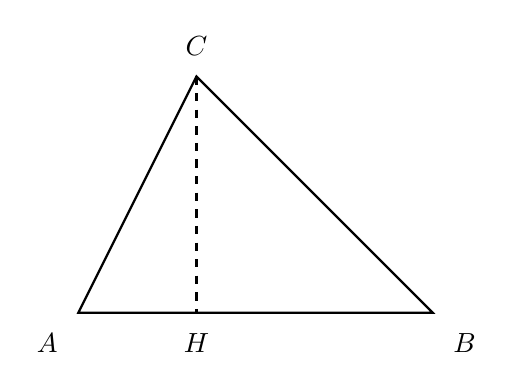
\begin{tikzpicture}[scale=3]
                        \coordinate (A) at (-0.5,0);
                        \coordinate (B) at (1,0);
                        \coordinate (C) at (0,1);
                        \coordinate (H) at (0,0);
                        \draw[thick]  (A) node[label=below left:$A$] {} -- (H) -- (B) node[label=below right:$B$] {} --  (C) node[label=above:$C$] {} -- cycle;
                        \draw[thick, dashed] (C) -- (H) node[label=below:$H$] {};
                    \end{tikzpicture}\hspace{2cm}
                    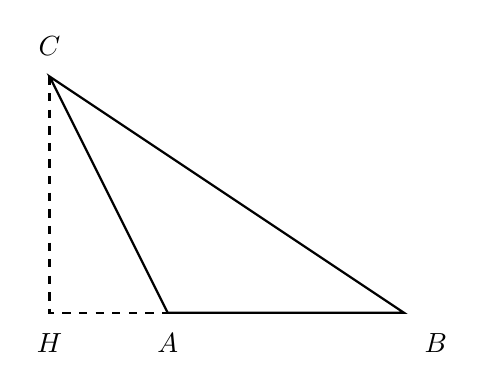
\begin{tikzpicture}[scale=3]
                        \coordinate (A) at (0.5,0);
                        \coordinate (B) at (1.5,0);
                        \coordinate (C) at (0,1);
                        \coordinate (H) at (0,0);
                        \draw[thick] (A) node[label=below:$A$] {} -- (B) node[label=below right:$B$] {} -- (C) -- cycle;
                        \draw[dashed, thick] (C) node[label=above:$C$] {} -- (H) node[label=below:$H$] {} -- (A);
                    \end{tikzpicture}
                    \[\overrightarrow{AB}\cdot\overrightarrow{AC}=\overrightarrow{AB}\cdot\overrightarrow{AH}\]\[=AB\times AH\qquad\text{ou}\qquad=-AB\times AH\]
                    \parbox{\linewidth}{\captionof{figure}{\centering Illustration du Produit Scalaire par Projeté Orthogonal}}
                \end{center}
            \end{SSpartie}
            \pagebreak
            \begin{SSpartie}{Définitions avec les Normes} 
                $\vec{u}\cdot\vec{v}=\dfrac{1}{2}\left(\lvert\lvert\vec{u}+\vec{v}\rvert\rvert^2-\lvert\lvert\vec{u}\rvert\rvert^2-\lvert\lvert\vec{v}\rvert\rvert^2\right)=\dfrac{1}{2}\left(\lvert\lvert\vec{u}\rvert\rvert^2+\lvert\lvert\vec{v}\rvert\rvert^2-\lvert\lvert\vec{u}-\vec{v}\rvert\rvert^2\right)$

                Ainsi, $\overrightarrow{AB}\cdot\overrightarrow{AC}=\dfrac{1}{2}\left(AB^2+AC^2-CB^2\right)$.
            \end{SSpartie}
            \begin{SSpartie}{Définition avec l'Angle} 
                $\vec{u}\cdot\vec{v}=\lvert\lvert\vec{u}\rvert\rvert\times\lvert\lvert\vec{v}\rvert\rvert\times\cos\,\left(\vec{u}~,\vec{v}\right)$
            \end{SSpartie}
        \end{Spartie}
        \begin{Spartie}{Propriétés} 
            Pour tous vecteurs $\vec{u}$, $\vec{v}$ et $\vec{w}$, et pour tout réel $\lambda$ : \[\vec{u}\cdot\vec{v}=\vec{v}\cdot\vec{u}\qquad\text{(symmétrie du produit scalaire)}\] \[\begin{drcases}\left(\lambda\vec{u}\right)\cdot\vec{v}=\lambda\times\left(\vec{u}\cdot\vec{v}\right)=\vec{u}\cdot\left(\lambda\vec{v}\right) \\ \vec{u}\cdot\left(\vec{v}+\vec{w}\right)=\vec{u}\cdot\vec{v}+\vec{u}\cdot\vec{w}\end{drcases}\text{(bilinéarité du produit scalaire)}\]
        \end{Spartie}
        \begin{Spartie}{Expressions Analytique du Produit Scalaire} 
            Dans un repère orthonormé de l'espace, $\vec{u}\,\left(x\,; y\,; z\right)$ et $\vec{v}\,\left(x'\,; y'\,; z'\right)$ étant deux vecteurs, alors : \[\vec{u}\cdot\vec{v}=xx'+yy'+zz'\] 
            \begin{SSpartie}{Démonstration} 
                On rappelle que $\lvert\lvert\vec{u}\rvert\rvert=\sqrt{x^2+y^2+z^2}$ :

                $\begin{aligned}[t]
                    \vec{u}\cdot\vec{v}&=\dfrac{1}{2}\left(\lvert\lvert\vec{u}+\vec{v}\rvert\rvert^2-\lvert\lvert\vec{u}\rvert\rvert^2-\lvert\lvert\vec{v}\rvert\rvert^2\right) \\
                    &=\frac{1}{2}\left(\left(x+x'\right)^2+\left(y+y'\right)^2+\left(z+z'\right)^2-\left(x^2+y^2+z^2\right)-\left(x'^2+y'^2+z'^2\right)\right) \\
                    &=\frac{1}{2}\left(2xx'+2yy'+2zz'\right) \\
                    &=xx'+y y'+z z'
                \end{aligned}$
            \end{SSpartie}
        \end{Spartie}
    \end{Gpartie}
    \pagebreak
    \begin{Gpartie}{Orthogonalité} 
        \begin{Spartie}{Vecteurs Orthogonaux} 
            \begin{SSpartie}{Définition} 
                Deux vecteurs de l'espace non nuls sont orthogonaux si deux droites qu'ils dirigent sont orthogonales.

                Par convention le vecteur nul est orthogonal à tout vecteur.

                \begin{SSSpartie}{Exemple} 
                    \begin{center}
                            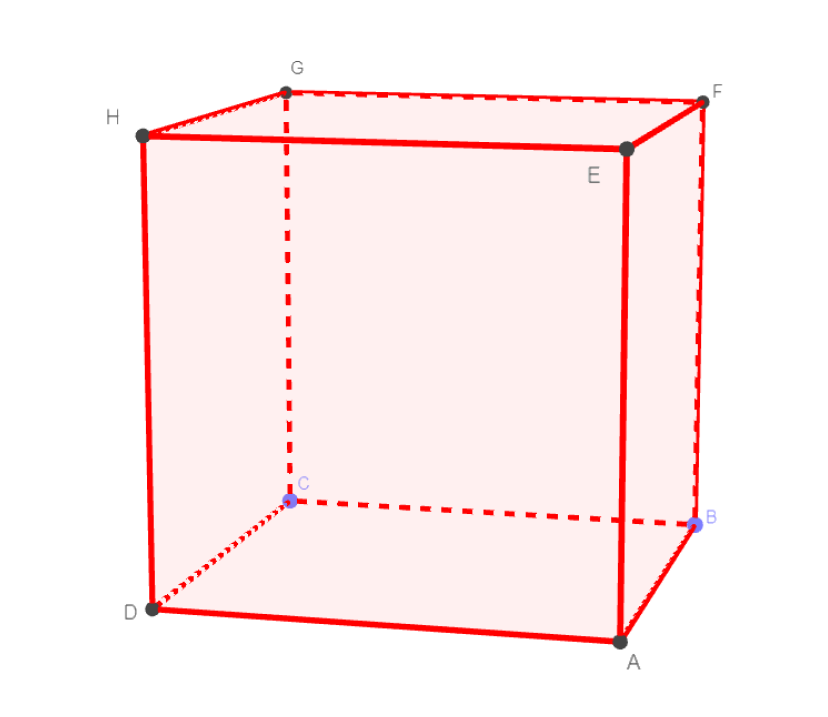
\includegraphics[width=5cm]{rsc/12fig2.png}
                            \[\overrightarrow{AB}\quad\text{et}\quad\overrightarrow{DH}\quad\text{sont orthogonaux}\]
                        \parbox{\linewidth}{\captionof{figure}{\centering Illustration de deux Vecteurs Orthogonaux}}
                    \end{center}
                \end{SSSpartie}
            \end{SSpartie}
            \begin{SSpartie}{Théorème} 
                Deux vecteurs $\vec{u}$ et $\vec{v}$ sont orthogonaux si et seulement si $\vec{u}\cdot\vec{v}=0$.
            \end{SSpartie}
            \begin{SSpartie}{Théorème} 
                Dans un repère orthonormé, deux vecteurs $\vec{u}~\left(x\,;y\,;z\right)$ et $\vec{v}~\left(x'\,;y'\,;z'\right)$ sont orthogonaux si et seulement si $xx'+yy'+zz'=0$. \quad(par définition analytique)
            \end{SSpartie}
        \end{Spartie}
        \pagebreak
        \begin{Spartie}{Vecteur Normal à un Plan} 
            \begin{SSpartie}{Définition} 
                Un vecteur \emph{normal} à un plan est un vecteur directeur d'une droite orthogonale à un plan.
    
                Un vecteur normal est par définition \emph{non nul}.
    
                \begin{center}
                        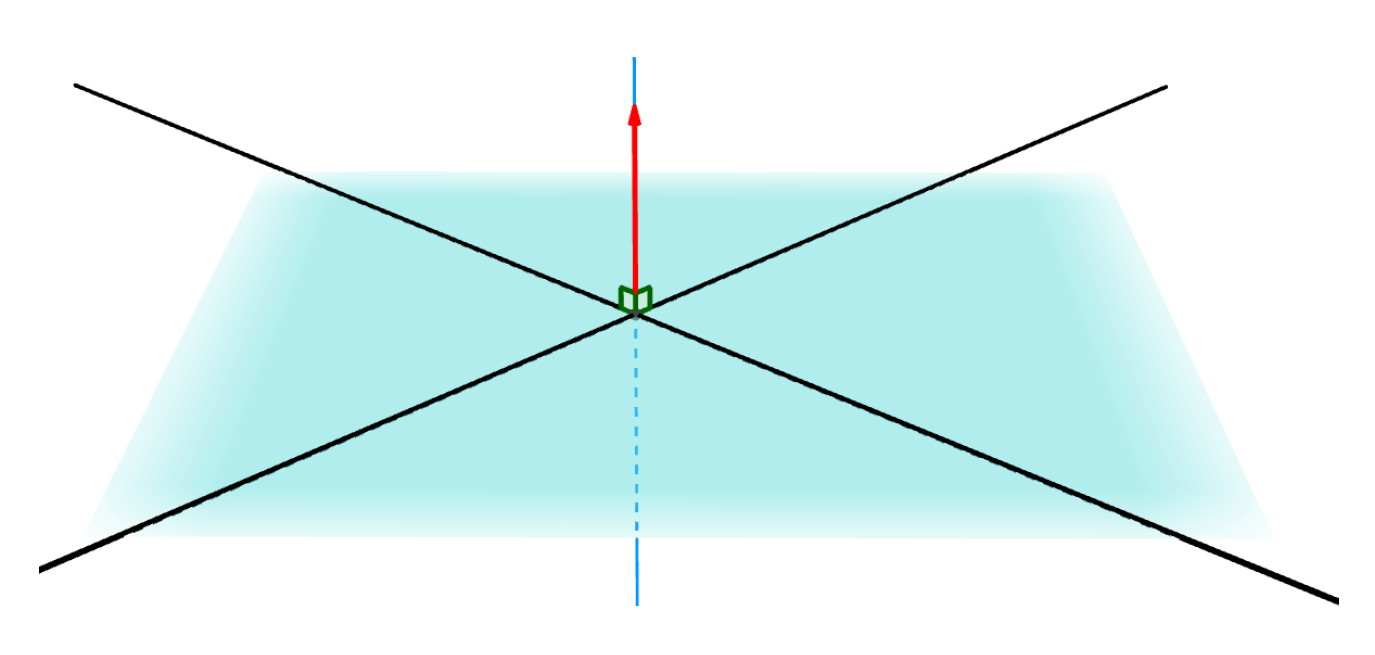
\includegraphics[width=5cm]{rsc/12fig3.png}
                    \parbox{\linewidth}{\captionof{figure}{\centering Illustration de la Définition}}
                \end{center}
            \end{SSpartie}
            \begin{SSpartie}{Caractérisation d'un Plan} 
                Un plan est caractérisé par \emph{un point} et un \emph{vecteur normal}.

                \begin{center}
                    
\includegraphics[width=5cm]{rsc/12fig4.png}
                    \parbox{\linewidth}{\captionof{figure}{\centering Caractérisation d'un Plan}}
                \end{center}
                
                                    Sur ce dessin, les deux plans ont le meme vecteur normal $\vec{n}$, donc la même direction. La position d'un plan sera déterminée par un point.
                
                                    On en déduit que deux plans parallèles admettent le meme vecteur normal, c'est-à-dire des vecteurs normaux colinéaires.
                \begin{SSSpartie}{Rappel} 
                    On peut aussi définir un plan par trois points non alignés, ou par deux droites sécantes (c'est-à-dire un point et deux vecteurs directeurs), ou, beaucoup plus rare, par deux droites parallèles non confondues.
                \end{SSSpartie}
            \end{SSpartie}
            \pagebreak
            \begin{SSpartie}{Théorème} 
                Le plan $\mathcal{P}$ qui passe par un point $A$ et de vecteur normal $\vec{n}$ est l'ensemble des point $M$ tels que $\overrightarrow{AM}\cdot\vec{n}=0$.\quad (admis ou définition d'un plan)

                \begin{center}
                    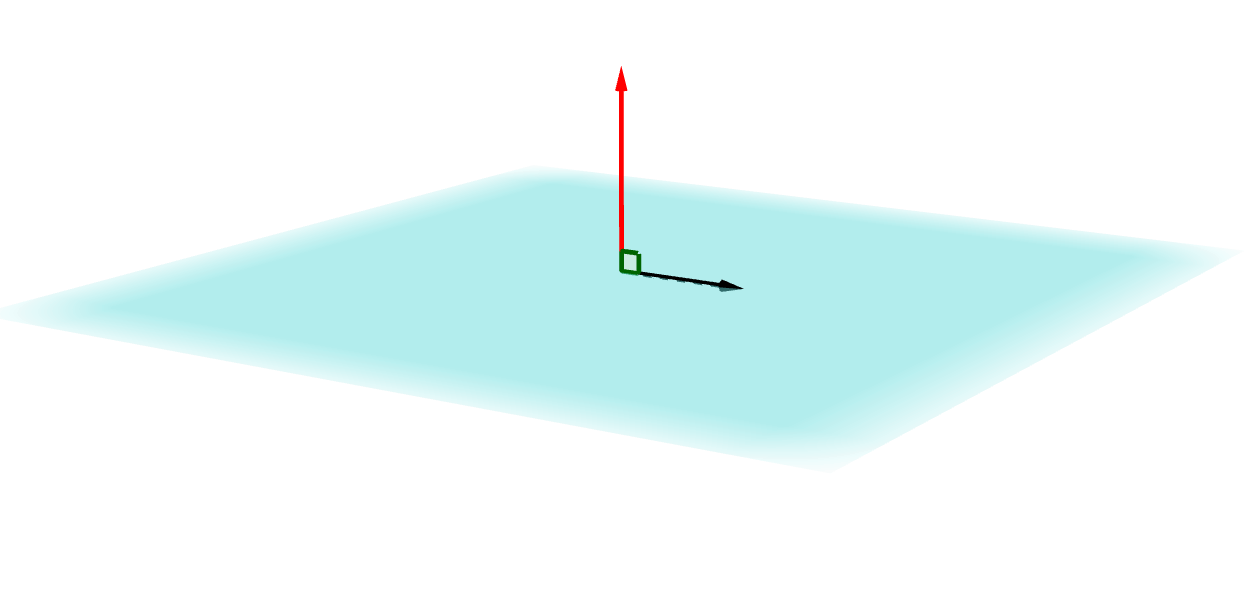
\includegraphics[width=5cm]{rsc/12fig5.png}
                    \parbox{\linewidth}{\captionof{figure}{\centering Illustration du Théorème}}
                \end{center}
            \end{SSpartie}
        \end{Spartie}
        \begin{Spartie}{Application (approfondissement)} 
            \begin{SSpartie}{Démonstration du Théorème} 
                \og Une droite est orthogonale à un plan si et seulement si elle est orthogonale à deux droites sécantes de ce plan. \fg
                \begin{itemize}[leftmargin=7ex]
                    \item[``$\implies$''] Si une droite est orthogonale à un plan, elle est orthogonale à toute droite de ce plan, en particulier deux droites sécantes de ce plan.
                    \item[``$\impliedby$''] Supposons qu'une droite $(d)$ est orthogonale à deux droites sécantes $d_1$ et $d_2$ du plan $\mathcal{P}$. Notons $A$ le point d'intersection de $d_1$ et $d_2$, et $\vec{u_1}$ et $\vec{u_2}$ deux vecteurs directeurs de $d_1$ et $d_2$.

                    Ainsi $\left(A\,;\vec{u_1}\,,\vec{u_2}\right)$ est un repère du plan $\mathcal{P}$, car $\vec{u_1}$ et $\vec{u_2}$ ne sont pas colinéaires.

                    Notons $\vec{n}$ un vecteur directeur de $(d)$. (on trace ci-dessous uniquement les vecteurs directeurs)
                    \vspace{-0.2ex}
                    \begin{center}
                        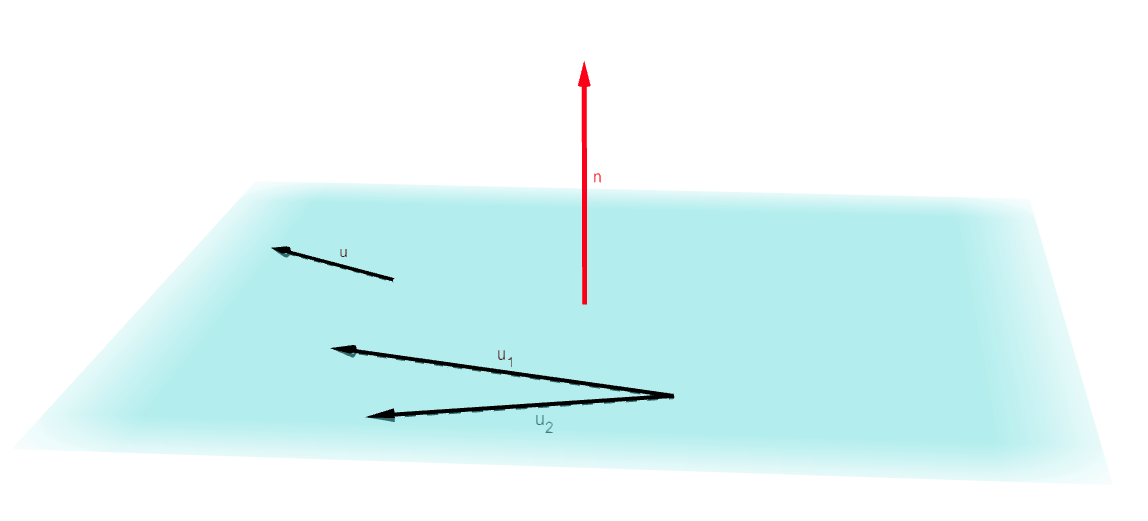
\includegraphics[width=5cm]{rsc/12fig6.png}
                        \parbox{\linewidth}{\captionof{figure}{\centering Représentation de la Situation}}
                    \end{center}
    
                    Alors, $\vec{n}$ est orthogonal à $\vec{u_1}$ et $\vec{u_2}$.

                    Soit une droite du plan $\mathcal{P}$, dont le vecteur directeur est $\vec{u}$.

                    Alors, il existe deux réels $\alpha$ et $\beta$ tels que $\vec{u}=\alpha\vec{u_1}+\beta\vec{u_2}$. \\ ($\vec{u}$, $\vec{u_1}$, $\vec{u_2}$ coplanaires)

                    Donc, $\vec{n}\cdot\vec{u}=\alpha\vec{n}\cdot\vec{u_1}+\beta\vec{n}\cdot\vec{u_2}=0$.\quad (car $\vec{n}$ orthogonal à $\vec{u_1}$ et $\vec{u_2}$)

                    Ainsi, $\vec{n}$ est orthogonal à $\vec{u}$, et donc $(d)$ est orthogonale à toute droite du plan~$\mathcal{P}$.\quad$\square$
                \end{itemize}
            \end{SSpartie}
        \end{Spartie}
        \begin{Spartie}{Plans Perpendiculaires} 
            Deux plans $\mathcal{P}_1$ et $\mathcal{P}_2$ admettant pour vecteurs normaux respectivement $\vec{n_1}$ et $\vec{n_2}$ sont perpendiculaires si et seulement si $\vec{n_1}\cdot\vec{n_2}=0$.

            \begin{center}
                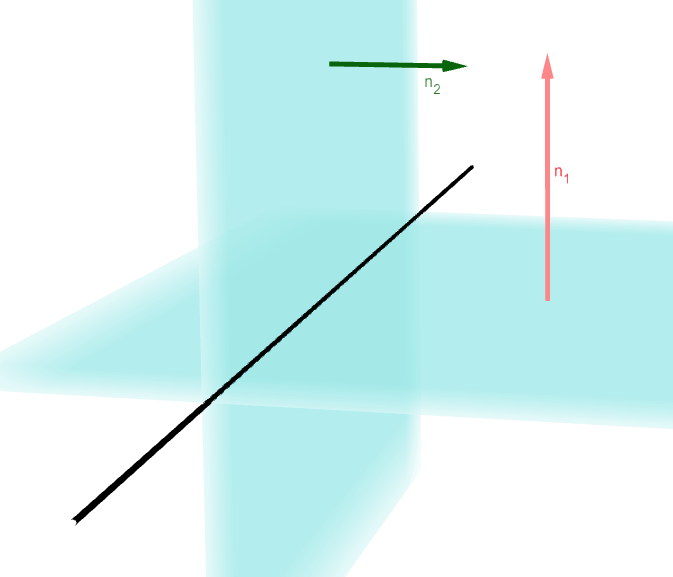
\includegraphics[width=5cm]{rsc/12fig7.png}
                \parbox{\linewidth}{\captionof{figure}{\centering Illustration de deux Plans Perpendiculaires}}
            \end{center}
        \end{Spartie}
    \end{Gpartie}
    \begin{Gpartie}{Projection Orthogonale d'un Point} 
        \begin{Spartie}{Projeté Orthogonal d'un Point sur un Plan} 
            \begin{SSSpartie}{Définition} 
                Le projeté orthogonal d'un point $A$ sur un plan $\mathcal{P}$ est l'intersection de $\mathcal{P}$ et de la droite orthogonale à $\mathcal{P}$ passant par $A$.
            \end{SSSpartie}
            \begin{SSSpartie}{Remarque} 
                Il existe une unique droite orthogonale (perpendiculaire) à $\mathcal{P}$ passant par $A$.
            \end{SSSpartie}
            \begin{SSSpartie}{Propriété} 
                Si $H$ est le projeté orthogonal du point $A$ sur le plan $\mathcal{P}$, le point $H$ est le point de $\mathcal{P}$ le plus proche de $A$. On l'appelle distance du point $A$ au plan $\mathcal{P}$.
                
                \begin{center}
                    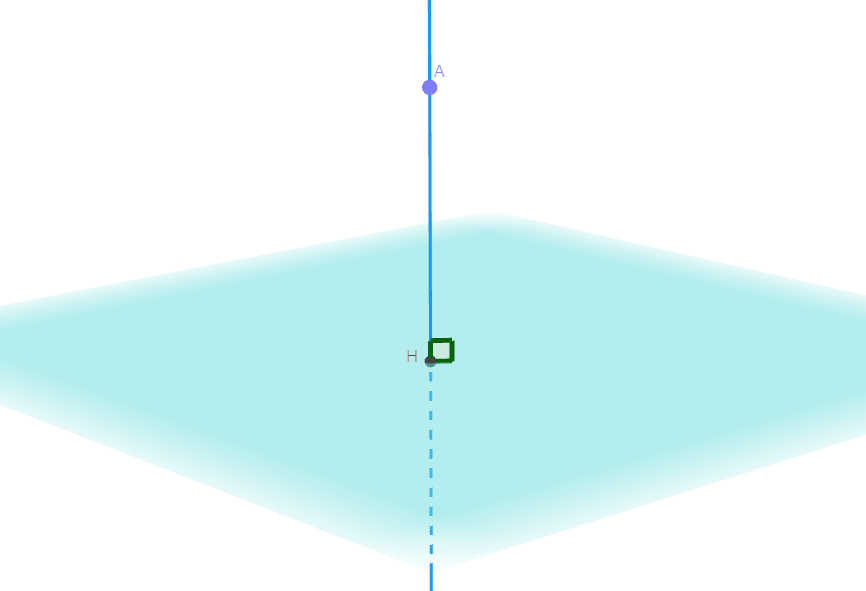
\includegraphics[width=5cm]{rsc/12fig8.png}
                    \parbox{\linewidth}{\captionof{figure}{\centering Illustration de la Propriété}}
                \end{center}

                \begin{SSSSpartie}{Démonstration} 
                    Soit $M$ un point de $\mathcal{P}$, comme $(AH)\perp\mathcal{P},~(AH)$ est orthogonale à toute droite de ce plan. \\ Donc $AMH$ est un triangle rectangle en $H$ et $AH^2=AM^2-MH^2\leq AM^2$.

                    Donc, pour tout point $M$ du plan, $AH\leq AM$.

                    \begin{center}
                        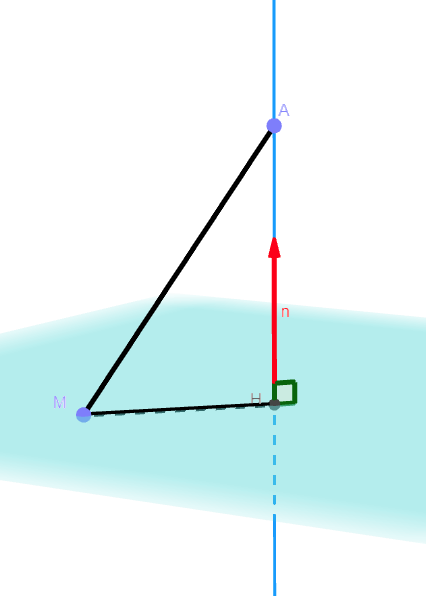
\includegraphics[width=5cm]{rsc/12fig9.png}
                        \parbox{\linewidth}{\captionof{figure}{\centering Illustration de la Démonstration}}
                    \end{center}    
                \end{SSSSpartie}
            \end{SSSpartie}
            \begin{SSSpartie}{Propriété} 
                Pour tout point $M$ du plan $\mathcal{P}$ : \[AH=\frac{\left\lvert\overrightarrow{AM}\cdot\vec{n}\right\rvert}{\lvert\lvert\vec{n}\rvert\rvert}=d~\left(~A~,~\mathcal{P}~\right)\]
                \begin{SSSSpartie}{Démonstration} 
                    $AH=AM\times\cos\,\left(~\widehat{MAH}~\right)$\quad (triangle rectangle AMH)

                    Or $\overrightarrow{AM}\cdot\vec{n}=AM\times\lvert\lvert\vec{n}\rvert\rvert\times\cos\,\left(\overrightarrow{AM}\,,\vec{n}\right)$.

                    Donc $\left\lvert\overrightarrow{AM}\cdot\vec{n}\right\rvert=AM\times\lvert\lvert\vec{n}\rvert\rvert\times\left\lvert\cos\,\left(\overrightarrow{AM}\,, \vec{n}\right)\right\rvert=AM\times\lvert\lvert\vec{n}\rvert\rvert\times\cos\,\left(~\widehat{MAH}~\right)$

                    Et donc, $\dfrac{\left\lvert\overrightarrow{AM}\cdot\vec{n}\right\rvert}{\lvert\lvert\vec{n}\rvert\rvert}=AH$
                \end{SSSSpartie}
            \end{SSSpartie}
        \end{Spartie}
        \begin{Spartie}{Projeté Orthogonal d'un Point sur une Droite} 
            \begin{SSpartie}{Définition} 
                Le projeté orthogonal d'un point $A$ sur une droite $(d)$ est l'intersection de $(d)$ et du plan orthogonal à $(d)$ passant par $A$.
            \end{SSpartie}
            \begin{SSpartie}{Remarque} 
                Il existe un unique plan orthogonal (perpendiculaire) à $(d)$ passant par $A$.
            \end{SSpartie}
            \begin{SSpartie}{Propriété} 
                Si $H$ est le projeté orthogonal du point $A$ sur la droite $(d)$, le point $H$ est le point de $(d)$ le plus proche de $A$. On l'appelle distance du point $A$ à la droite $(d)$.
            \end{SSpartie}
        \end{Spartie}
    \end{Gpartie}
\end{document}